\section{Right words, wrong dialect}\label{sec:dissociation}

\Cref{tab:bakeoff} and \cref{fig:dissociation} give the bake-off on the 32 non-digit Egyptian sentences, each spoken
in three Egyptian voices. The quantities a practitioner would look at first and the dialect do not agree.

\begin{table}[t]
\centering\small
\caption{Bake-off on colloquial Egyptian text (32 sentences $\times$ 3 voices $= 96$ utterances per system; one seed).
CER from Whisper large-v3 with a two-way bootstrap interval over texts and voices. ``Labelled Egyptian'': share of
outputs whose top label is Egyptian under each dialect classifier (real colloquial Egyptian speech:
\R{cal:lahgtna:c1pct} and \R{cal:lahgtna:c2pct}; dialect bar \R{sel:bar:c1} and \R{sel:bar:c2}). Listener: the author's
informal check on six sentences per system, rated Egyptian / partly / not Egyptian. $^\dagger$Non-commercial weights,
measured for reference only. Below the line: a diagnostic loader of Chatterbox V3. Intervals for every column are in
\cref{tab:bakeoff_full}.}
\label{tab:bakeoff}
\begin{adjustbox}{max width=\linewidth}
\rawinput{generated/tab_bakeoff.tex}
\end{adjustbox}
\end{table}

\begin{figure}[t]
\centering
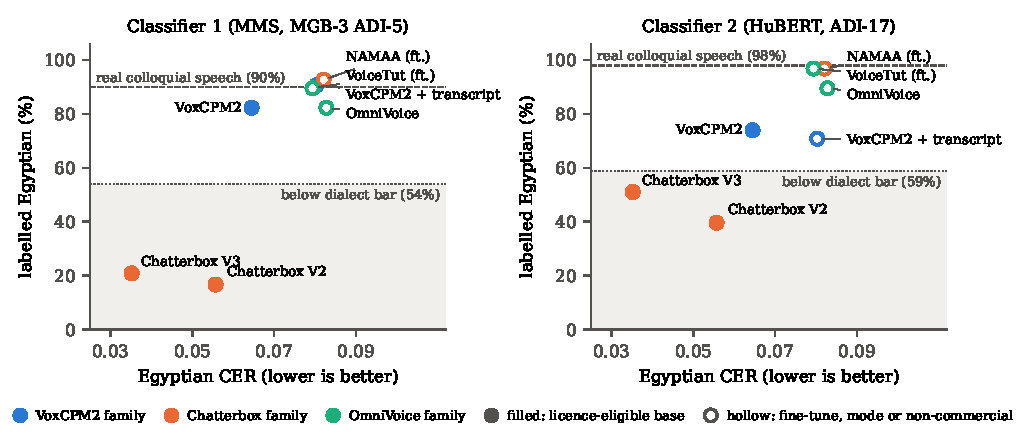
\includegraphics[width=\linewidth]{figures/dissociation.pdf}
\caption{Egyptian CER against the share of outputs labelled Egyptian, under two independent dialect classifiers
(bake-off, 96 utterances per system). Shaded: below the dialect bar, 60\% of the share on real colloquial speech. The
two lowest-CER systems are the two least Egyptian. Off the CER scale and not shown: \R{fig:offscale}.}
\label{fig:dissociation}
\end{figure}

\paragraph{Lowest CER, least Egyptian}
\cbthree has the lowest CER of all systems (\R{bk:cb-v3:cer}), and Chatterbox~V2 the second lowest
(\R{bk:cb-v2:cer}). Classifier~1 labels only \R{bk:cb-v3:c1pct} and \R{bk:cb-v2:c1pct} of their outputs Egyptian,
against \R{cal:lahgtna:c1pct} for real colloquial Egyptian speech; most of the rest is labelled Levantine
(\R{lab:cb-v3:Levantine} for V3), Gulf (\R{lab:cb-v3:Gulf}) or MSA (\R{lab:cb-v3:MSA}). \vox has a higher CER
(\R{bk:voxcpm2:cer}), with an interval that overlaps \cbthree's, and is labelled Egyptian \R{bk:voxcpm2:c1pct} of the
time. Speaker similarity and predicted quality do not separate the bases either: \cbthree has the highest DNSMOS of
the three eligible bases and Chatterbox~V2 the highest similarity.

\paragraph{What each metric would choose}
Point estimates on 96 utterances could pick a winner by chance, so we ask how often a selection rule fails, not
whether it failed once. We resample texts and voices (two-way bootstrap, \R{sel:B} resamples, the same draw for every
system), apply each rule in every resample, and record whether the chosen system clears the dialect bar in that
resample (\cref{tab:selection}). Among the three licence-eligible bases, the decision G1 actually had to make, every
standard metric picks a Chatterbox model: lowest CER picks \R{sel:eligible:cer:pick} in \R{sel:eligible:cer:pickshare}
of resamples, and the chosen system fails the bar in \R{sel:eligible:cer:fail1} of resamples under classifier~1 and
\R{sel:eligible:cer:fail2} under classifier~2; highest similarity fails in \R{sel:eligible:ecapa:fail1} and
\R{sel:eligible:ecapa:fail2}, highest predicted quality in \R{sel:eligible:dnsmos:fail1} and
\R{sel:eligible:dnsmos:fail2}. Lowest CER among the systems that clear the bar picks \vox in
\R{sel:eligible:amended:pickshare} of resamples. Across all nine configurations, which include Egyptian fine-tunes and
non-commercial models, lowest CER still fails the bar in \R{sel:all:cer:fail1} of resamples (classifier~1), while
highest similarity happens to pick OmniVoice, a non-commercial model that clears it. The failure is therefore not that
every metric always points away from the dialect, but that none of them carries information about it, so which system
they pick depends on what else is in the pool.

\begin{table}[t]
\centering\small
\caption{What each selection rule picks, over \R{sel:B} two-way bootstrap resamples of the bake-off (texts and voices
resampled, the same draw for every system). Pick: the rule's choice on the full data. Picked: share of resamples in
which the rule chose that system. Fails bar: share of resamples in which the rule's choice, whichever it was, falls
below the dialect bar (\R{sel:bar:c1} for classifier~1, \R{sel:bar:c2} for classifier~2). Last row: the amended G1.
$^\dagger$Non-commercial weights.}
\label{tab:selection}
\begin{adjustbox}{max width=\linewidth}
\rawinput{generated/tab_selection.tex}
\end{adjustbox}
\end{table}

\paragraph{Three seeds on held-out sentences}
The bake-off has one seed per utterance. On the 24 held-out Egyptian sentences, each generated with three seeds, the
paired comparison of \vox and \cbthree gives a CER difference of \R{pt:voxcpm2_minus_cb-v3:egy_main:cer_best:diff}
(95\% CI \R{pt:voxcpm2_minus_cb-v3:egy_main:cer_best:ci}) and a similarity difference of
\R{pt:voxcpm2_minus_cb-v3:egy_main:sim_ecapa:diff} (CI \R{pt:voxcpm2_minus_cb-v3:egy_main:sim_ecapa:ci}): the two
cannot be told apart. DNSMOS prefers \cbthree (\R{pt:voxcpm2_minus_cb-v3:egy_main:mos_p808:diff}, CI
\R{pt:voxcpm2_minus_cb-v3:egy_main:mos_p808:ci}). The Egyptian share separates them by
\R{pt:voxcpm2_minus_cb-v3:egy_main:c1:diff} under classifier~1 (CI \R{pt:voxcpm2_minus_cb-v3:egy_main:c1:ci},
$\R{pt:voxcpm2_minus_cb-v3:egy_main:c1:pholm}$) and \R{pt:voxcpm2_minus_cb-v3:egy_main:c2:diff} under classifier~2
(CI \R{pt:voxcpm2_minus_cb-v3:egy_main:c2:ci}, $\R{pt:voxcpm2_minus_cb-v3:egy_main:c2:pholm}$). With three seeds,
lowest CER picks \cbthree in \R{sel3:cer:cbv3} of resamples and highest DNSMOS in \R{sel3:dnsmos:cbv3}.

\paragraph{No relation across systems}
Across the nine configurations, Spearman's rank correlation between CER and the Egyptian share is
\R{sel:rhoc1} under classifier~1 (bootstrap 95\% interval \R{sel:rhoc1:ci}) and \R{sel:rhoc2} under classifier~2
(\R{sel:rhoc2:ci}). Nine systems cannot rule out a moderate relation in either direction, and we do not rest the claim
on these coefficients; the selection analysis above is the direct test.

\paragraph{Two classifiers, trained on different data, agree}
The finding could be an artefact of one classifier. Classifier~2 was trained on different speech (YouTube rather
than broadcast) with a different backbone and label set. It is more generous to every system, but it ranks the
systems in nearly the same order (Spearman $\rho=\R{rank:c1c2:rho}$, $p=\R{rank:c1c2:p}$), and under it too both
Chatterbox bases fall below the dialect bar while \vox clears it. Per utterance the classifiers agree moderately
(Cohen's $\kappa=\R{kappa:real}$ on calibration speech, \R{kappa:gen} on generated speech), so we rely on system-level
shares, not on single labels.

\paragraph{Not an artefact of the reference voices}
FLEURS references are read and mostly MSA in register, so a system could sound un-Egyptian because it copies the
reference's register. Splitting the bake-off by the dialect of the reference clip itself does not remove the gap under
classifier~1: with the \R{ref:egy:nvoices} references that both classifiers label Egyptian, \cbthree is labelled
Egyptian \R{ref:cb-v3:egy:c1} of the time and \vox \R{ref:voxcpm2:egy:c1}; with the \R{ref:msa:nvoices} references
labelled MSA by both, \R{ref:cb-v3:msa:c1} and \R{ref:voxcpm2:msa:c1}. Classifier~2 is more sensitive to the reference:
with Egyptian references it labels \cbthree Egyptian \R{ref:cb-v3:egy:c2} of the time against \R{ref:voxcpm2:egy:c2}
for \vox, a smaller gap than with MSA references (\R{ref:cb-v3:msa:c2} against \R{ref:voxcpm2:msa:c2}). Two or three
voices per group make these intervals wide (\texttt{selection.md}); the direction holds in every cell, but how much a
colloquial reference helps a model without Egyptian training data is a question for colloquial reference recordings
(\cref{sec:limitations}).

\paragraph{The ear agrees, informally}
In an informal check of six sentences per system, with names hidden and order shuffled, the author, a native Egyptian
speaker, rated both Chatterbox bases ``not Egyptian'' on \R{lt:cb-v3:not} sentences, and \vox ``not Egyptian'' on none
(Egyptian on \R{lt:voxcpm2:egy}, partly on \R{lt:voxcpm2:mid}). One listener who knew the hypothesis, rating six
sentences, settles nothing; we report the check because it agrees with both classifiers on the decision that matters,
and we do not count it as evidence on its own. A multi-listener test is the next step (\cref{sec:limitations}).

\paragraph{Why}
The pattern fits the training data rather than the architecture. The three Chatterbox-based systems without documented
Egyptian training data (V3, V2 and the lahgtna fine-tune) are labelled Levantine more than anything else
(\R{lab:chat:lev} of their outputs together), while NAMAA, a Chatterbox fine-tune on Egyptian speech, is labelled
Egyptian \R{bk:namaa:c1pct} of the time. A recogniser trained mostly on MSA and pan-Arabic data transcribes Levantine-
or MSA-accented Egyptian sentences correctly: the words survive, the dialect does not, and CER cannot see the
difference. Accent may even help CER, since speech closer to the recogniser's training distribution is easier to
transcribe. Our data cannot separate these explanations, but neither rescues CER as a selection criterion.

\paragraph{Consequence for model selection}
A selection rule that ranks by intelligibility, similarity or predicted quality, as our own pre-registered gate G1 did
with CER, picks a base without regard to the dialect. For any product whose purpose is to speak a dialect, these
metrics have to be paired with a dialect measure calibrated on real dialectal speech and, where possible, native
listeners, and the bar should be fixed relative to the same measure on real speech, since classifiers differ in how
generous they are.
